\documentclass[oneside,a4paper,12pt]{article}
\usepackage{graphicx}
\usepackage[section]{placeins}
\usepackage{listings}
\graphicspath{{~/templates/}, {../images/}}

\makeindex
\begin{document}
	\begin{titlepage}
		\includegraphics[width=4cm]{logopopo.png}
		\hspace*{\fill}
		\includegraphics[width=6cm]{univlille.png}
		
		\begin{center}
			\vspace{1cm}
			\textbf{TP Variation de Vitesse}\\
			\textbf{TP2 }\\
			\vspace{1cm}
			\textbf{Valentin DOSIAS, Maxence NEUS}\\
			\vspace{\fill}
			\textbf{Novembre 2021}\\
		\end{center}
	\end{titlepage}
	
	\tableofcontents
	
	\section{Introduction}
	\paragraph{}
	L’objectif de ce TP est de mettre en évidence les différentes variables mises en jeu lors d’une conversion électromagnétique ainsi que les interactions et les transferts énergétiques entre les différents composants de puissance. Nous étudierons ces variables sur une maquette de VAL (véhicule automatique léger) composée de deux moteurs à courant continu dont l’un génère la force du moteur du véhicule et l’autre génère la force d’un couple résistant ou non (monté ou descente du véhicule).
		
	\newpage
			
	\section{Manipulation}
	
	
	\subsection{Causalités Internes De La Machine}
	
		Nous avons eu un problème avec l’enregistrement de nos courbes, elles se sont enregistrées sous le mauvais format nous n’avons pas pu les avoir tels que les captures d’écrans étaient. Nous les avons donc retracées sur papier ou extrait avec un logiciel Tektronic mais une seule courbe sur les deux prises par l’oscillo a pu être extraite.
		
		\begin{figure}[h]
			\centering
			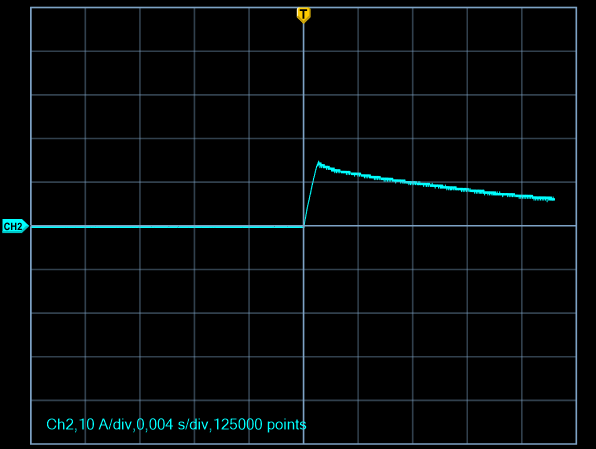
\includegraphics[width=8cm]{capture-1.PNG}
			\caption{Courant de la machine}
		\end{figure}
		\begin{figure}[h]
			\centering
			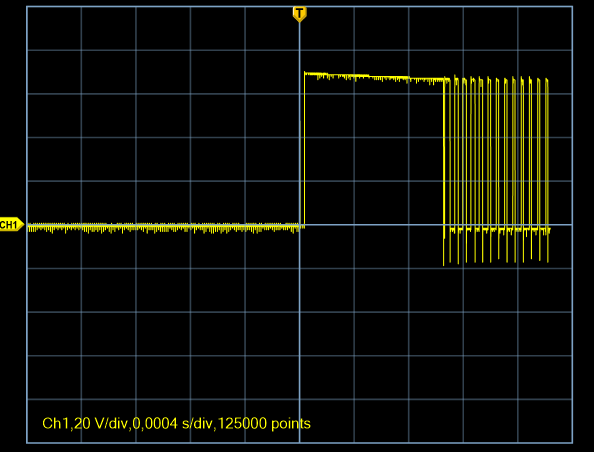
\includegraphics[width=8cm]{capture-3.PNG}
			\caption{Tension hacheur}
		\end{figure}
	
		\newpage
		
		Sans forcément superposer, les graphes et en étudiant leur échelle de temps nous pouvons logiquement déduire laquelle est la cause et laquelle est la conséquence. Nous voyons que la tension s’établit sur une légère fraction d’une division de 0.0004 seconde alors que le courant s’établit en environ 1⁄4 d'une division de 0.004 seconde soit 0.001 seconde ce qui est très largement supérieur au temps de la tension. Nous pouvons en déduire  que la tension est la cause et le courant la conséquence (l’effet).
		
		\begin{figure}[h]
			\centering
			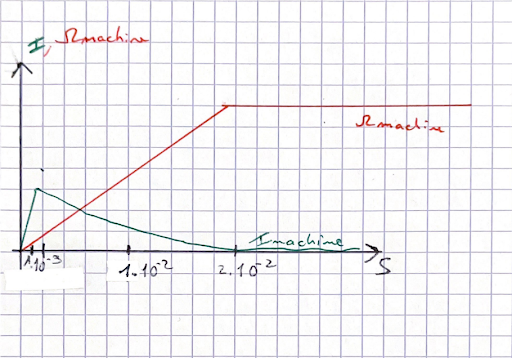
\includegraphics[width=10cm]{part1.png}
			\caption{Allure des courbes superposées}
		\end{figure}
		
		Pour la vitesse, nous n’avons pas réussi à récupérer la courbe. Cependant, nous avons mesuré un temps de réponse indicielle d’environ 0.02 sec ce qui est aussi largement supérieur à la réponse du courant la vitesse de la machine est la conséquence du courant et donc du couple électromagnétique e de la machine car le couple électromagnétique et le courant délivré par la machine sont proportionnelles.
		$$ I_{m}=C_{em}*k_{\phi} $$
		Nous pouvons donc classer les variables dans l’ordre, nous avons la réception de la consigne soit $\Omega_{ref}$ , le générateur délivre donc une tension Uhach à la machine qui génère un courant entraînant un couple électromagnétique qui vient donc entraîner le bras du moteur à courant continu à une certaine vitesse.
		
		
	\newpage
	\subsection{Fonctionnement à tension d'alimentaion constante}
	
		Dans cette partie, on fixe la tension d'alimentation et on va observer l'influence de du couple de résistance de la génératrice sur le courant absorbé par la machine et la vitesse de rotation.
		
		
		On fixe U=25V.
		
		\begin{figure}[h]
			\centering
			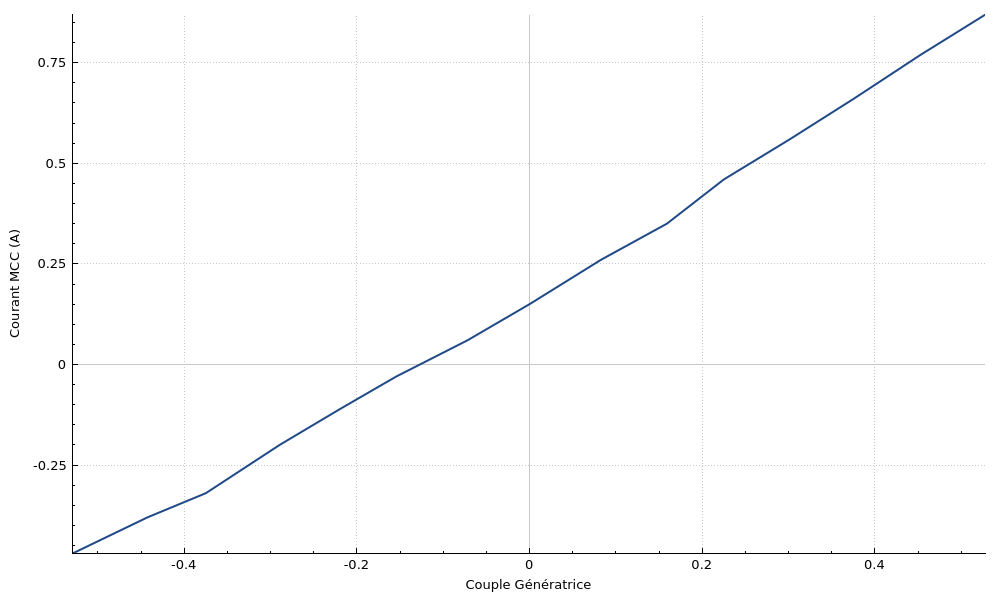
\includegraphics[width=9cm]{PlotImachdeCgene.png}
			\caption{Courant absorbé par la MCC}
		\end{figure}
	
		On voit ici que le courant absorbé suit une loi afine du type $$ I=\frac{C}{k_{\phi}} + C_{r} $$
		
		Avec $C_{r}$ le couple de résistance associé aux pertes méchaniques qu'on peut identifier ici à environ 0.2 Nm.

		\begin{figure}[h]
			\centering
			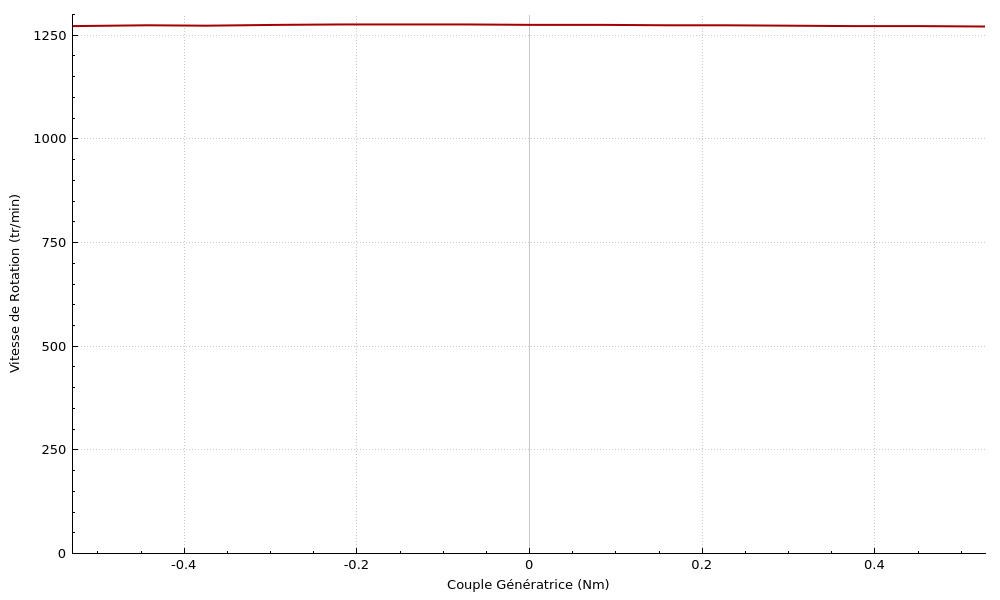
\includegraphics[width=9cm]{PlotNdeCgene.png}
			\caption{Vitesse de la MCC}
		\end{figure}
	
		Comme on pouvait l'attendre, la vitesse du moteur ne dépends pas du couple résistant mais bien uniquement de la tension d'alimentation.
	
	\subsection{Fonctionnement à couple résistant constant}
	
	Dans cette partie, on fixe maintenant le couple résistant appliqué à la machine.
	On fixe cette fois C=0.5Nm.
	
	On observe cette fois le courant absorbé par la machine en fonction de la tension d'alimentation.
	
	\begin{figure}[h]
		\centering
		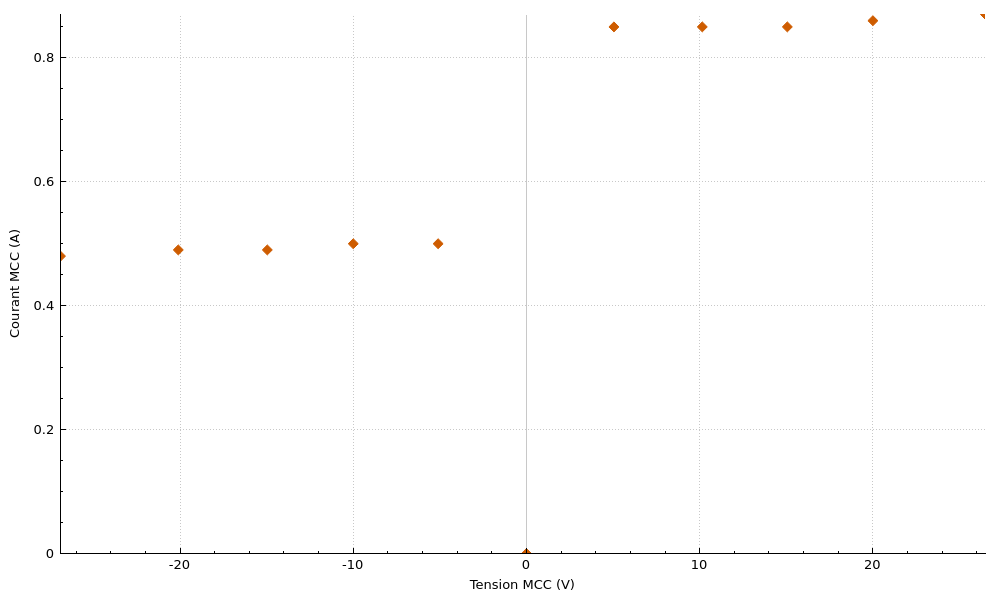
\includegraphics[width=9cm]{PlotIdeU.png}
		\caption{Courant absorbé par la MCC}
	\end{figure}

	On voit le courant absorbé reste constant dans un sens de rotation, ce qui colle avec ce qu'on attend d'après le cours. En effet le courant est uniquement fonction du couple résistant qui lui est appliqué.
	
	\subsection{Asservissement de vitesse}
	
	Dans le cadre de la commade du metro, une commande en tension simple nous apporte une vitesse constante comme vu en partie 2. La seule différence vient du courant absorbé qui varie largement en fonction du couple résistant (qui correspond aux changements deans la pente des rails).\\
	Il faut donc maintenir une tension d'alimentation constante pour assurer une vitesse du metro constante.\\
	
	\newpage
	\subsection{Bilan énergétique de divers modes de fonctionnement}
		
	Dans cette partie, on commande le moteur en marche avant et marche arrière de manière periodique. Cette commande nous permet d'observer les points de fonctionnement moteur marche avant et marche arrière (respectivement les cadrants supérieur droit et inférieur gauche).
	
	Pour observer ces points de fonctionnement, on mesure la vitesse de rotation du moteur et le courant absorbé par le moteur qui représente l'image du couple moteur.\\
	Ces mesures sont visualisées en mode XY pour visualiser le plan Vitesse/Couple.\\
	
	\begin{figure}[h]
		\centering
		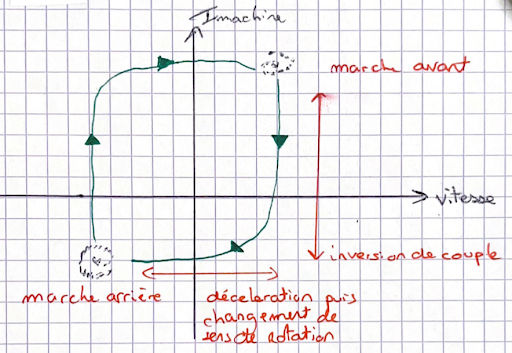
\includegraphics[width=11cm]{partFinal.png}
		\caption{Allure des points de fonctionnement}
	\end{figure}

	On peut utiliser les considérations de causalité étudiées en partie 1 pour déterminer les déplacements du point de fonctionnement lors des changements de commande.\\
	Comme vu précedement, le courant $I_{mach}$ varie bien plus rapidement que la vitesse et on passe donc par un comportement de freinage avant d'accelerer à nouveau pour atteindre le nouveau point de fonctionnement (symbolisé par les flèches vertes sur le schéma).\\
	On a pu également observer que les oscillations des grandeurs amènent un mouvement en spirale du point de fonctionnement autour du point ciblé.\\
		
	
\end{document}